\documentclass[aspectratio=169]{beamer}
\usepackage{colortbl}
\usepackage{booktabs}
\usepackage{tabularx}
\usepackage{pifont}
\usepackage{tikz}
\usepackage{setspace}
\usetikzlibrary{arrows,calc,fit,backgrounds,external,positioning}

\usepackage{pgfplots}
\usepackage{pgfplotstable}
\pgfplotsset{compat=1.15}
\usepgfplotslibrary{dateplot,fillbetween}

\usepackage{xcolor}
\definecolor{normalred}{HTML}{EA1908}
\definecolor{darkred}{HTML}{AF0001}
\definecolor{burgundy}{HTML}{75000B}
\definecolor{lightgreen}{HTML}{CBF5DB}

\definecolor{mediumblue}{HTML}{1FA3B3}
\definecolor{mediumblue1}{HTML}{61D9E5}
\definecolor{mediumblue2}{HTML}{0C5058}

\definecolor{lightblue}{HTML}{7DC7CD}
\definecolor{lightblue1}{HTML}{B2DCE2}
\definecolor{lightblue2}{HTML}{41A9B5}

\definecolor{yellow}{HTML}{E4E102}
\definecolor{yellow1}{HTML}{FFFE8F}
\definecolor{yellow2}{HTML}{717200}

\mode<presentation>
{
  \usetheme{default}
  % ou autre ...Copenhagen

%  \setbeamercovered{transparent}
%  \setbeamertemplate{footline}[frame number]
  \setbeamertemplate{footline}{%
  \raisebox{5pt}{\makebox[\paperwidth]{\hspace{15cm}\makebox[10pt]{\scriptsize  \insertframenumber/\inserttotalframenumber\phantom{1}}}}}
  \setbeamertemplate{navigation symbols}{}
  % ou autre chose (il est galement possible de supprimer cette ligne)
%  \setbeamerfont{frametitle}{series=\bfseries}
  \usefonttheme{default}
 
\setbeamercolor{part title}{fg=mediumblue}
\setbeamertemplate{itemize item}{\color{lightblue}$\blacksquare$}
\setbeamertemplate{itemize subitem}{\color{lightblue}$\blacktriangleright$}

\setbeamercolor*{enumerate item}{fg=lightblue}
\setbeamercolor*{enumerate subitem}{fg=lightblue2}
\setbeamercolor*{enumerate subsubitem}{fg=lightblue1}

%\setbeamertemplate{section title}{\insertsectionhead}
%\setbeamercolor{section title}{mediumblue}
}

\defbeamertemplate{footline}{mydefault}{%
  \raisebox{5pt}{\makebox[\paperwidth]{\hspace{15cm}\makebox[10pt]{\scriptsize  \insertframenumber/\inserttotalframenumber\phantom{1}}}}
}

\defbeamertemplate{footline}{emptyfootline}{%
}

\defbeamertemplate{background canvas}{mydefaultbackground}{%
  \begin{tikzpicture}[remember picture,overlay]
    % Header: top of image stuck to top of page
    \node[anchor=north west, inner sep=0pt] at (current page.north west) {%
      
\includegraphics[width=\paperwidth]{frame/Header.png}%
    };
    % Footer: bottom of image stuck to bottom of page
    \node[anchor=south west, inner sep=0pt] at (current page.south west) {%
      
\includegraphics[width=\paperwidth]{frame/Footer.png}%
    };
  \end{tikzpicture}%
}

\defbeamertemplate{background canvas}{titleframebackground}{%

\includegraphics[width=\paperwidth, height=\paperheight]{frame/TitlePage.png}%
}

\defbeamertemplate{background canvas}{titleframebackground2}{%

\includegraphics[width=\paperwidth, height=\paperheight]{frame/TitlePage2.png}%
}


\setbeamercolor{section in head/foot}{fg=mediumblue2,bg=}
\setbeamercolor{frametitle}{fg=lightblue,bg=}

\setbeamerfont{section title}{size=\large,series=\bfseries}
\setbeamerfont{frametitle}{size=\Large,series=\bfseries}


% --- custom frametitle template ---
\defbeamertemplate{frametitle}{custom}{%
\vspace{3ex}
% section number + section title
  \hspace{-1.5em}\begin{beamercolorbox}[wd=\paperwidth,ht=2.5ex,dp=1.5ex,sep=0.6ex,right]{section in head/foot}%
    \usebeamerfont{section title}%
    % move left (-0.5em) and up (raise by 0.3ex)
    \raisebox{0ex}[0pt][0pt]{\textbf{\thesection .~\insertsection}}%
  \end{beamercolorbox}%

    % --- Horizontal rule (TikZ overlay) ---
    \nointerlineskip
    \vspace*{-0.5ex}%
    \begin{tikzpicture}[remember picture,overlay]
      \draw[mediumblue2, line width=0.6pt] 
        ([xshift=0pt,yshift=-38pt]current page.north west) -- 
        ([xshift=0pt,yshift=-38pt]current page.north east);
    \end{tikzpicture}

  \vspace*{-0.4ex}%
  % frame title, right-aligned (light blue)
  \begin{beamercolorbox}[wd=\paperwidth,ht=1ex,dp=1.5ex,sep=0.6ex,left]{frametitle}%
    \usebeamerfont{frametitle}%
    \textbf{\insertframetitle}%
  \end{beamercolorbox}%
  \vspace{-6ex}%
}

%\defbeamertemplate{frametitle}{emptyframetitle}{}
% activate it
%\setbeamertemplate{frametitle}[custom]

% Default frame
\BeforeBeginEnvironment{frame}{%
\setbeamertemplate{background canvas}[mydefaultbackground] %
  \setbeamertemplate{frametitle}[custom]%
    \setbeamertemplate{footline}[mydefault]
}

% Title frame
\makeatletter
\define@key{beamerframe}{titleframe}[true]{%
  \setbeamertemplate{background canvas}[titleframebackground]
  \setbeamertemplate{footline}[emptyfootline]%
}
\makeatother

% End frame
\makeatletter
\define@key{beamerframe}{endframe}[true]{%
  \setbeamertemplate{background canvas}[titleframebackground2]
  \setbeamertemplate{footline}[emptyfootline]%
  %\setbeamertemplate{frametitle}[emptyframetitle]%
}
\makeatother

% Empty frame
\makeatletter
\define@key{beamerframe}{emptyframe}[true]{%
  \setbeamertemplate{background canvas}[mydefaultbackground]
%  \setbeamertemplate{frametitle}[]%
  \setbeamertemplate{footline}[mydefault]
}
\makeatother

\usepackage{textcomp} 

\usepackage[utf8]{inputenc}
\usepackage{t1enc}
\def\magyarOptions{defaults=hu-min}
\usepackage[magyar]{babel}

\usepackage{multirow,tabularx}
%\usepackage{lmodern} %%Ne pas changer la police celle-ci est bien 
\usepackage[final]{animate}
\usepackage{amsmath}
\usepackage{siunitx}
\sisetup{print-unity-mantissa = false}

\usepackage{pgfplots}
\usepackage{pgfplotstable}
\pgfplotsset{compat=1.15}
%\usepgfplotslibrary{dateplot}
%\usepgfplotslibrary{units}

\newcommand{\blocktext}[2]{%
\textbf{#1}\\
\small #2
}

\newlength{\ydist}
\setlength{\ydist}{0.04\textheight}

\newlength{\deltadist}
\setlength{\deltadist}{0.03\ydist}

\tikzset{>=stealth'}

\setbeamercolor{titlelike}{parent=structure,fg=mediumblue}
\setbeamercolor{frametitle}{parent=structure,fg=mediumblue}
\setbeamercolor{link}{parent=structure,fg=lightblue}
\newcommand{\gn}[1]{{\usebeamercolor[fg]{titlelike}#1}}
\newcommand{\highlight}[1]{{\bfseries\usebeamercolor[mediumblue2]{titlelike}#1}}

\usepackage{hyperref}
\hypersetup{colorlinks=true,linkcolor=mediumblue2,urlcolor=lightblue2}

\setbeamerfont{title}{family=\sffamily}
\setbeamerfont{author}{family=\sffamily}
\setbeamerfont{institute}{family=\sffamily}
\setbeamerfont{date}{family=\sffamily}
\setbeamerfont{frametitle}{series=\scshape}
\setbeamerfont{framesubtitle}{family=\sffamily}
\setbeamerfont{caption}{family=\sffamily}
\setbeamercolor{normal text}{bg=white,fg=black}

\usepackage{multicol}
\usepackage{multirow}

\setbeamercolor{block body}{fg=lightblue, bg=white!0!white}
\setbeamercolor{coloredboxstuff}{fg=lightblue,bg=white!0!white}

\usefonttheme[onlymath]{serif}

\newcommand{\hly}[1]{\colorbox{yellow}{\parbox{\textwidth}{#1}}}

\graphicspath{{./figures/}}

\begin{document}


{
\setbeamertemplate{footline}{}
\begin{frame}[titleframe,noframenumbering]
\begin{LARGE}
\color{white}
\MakeUppercase{\textbf{72.~Vándorgyűlés}}
\end{LARGE}

\vspace{-0.5ex}
\color{mediumblue}\rule{0.52\textwidth}{1.5pt} \\

\begin{Large}
Konferencia és Kiállítás
\end{Large}

\vspace{3.5ex}
\hspace{-0.5cm}
\begin{flushleft}
\begin{LARGE}
\textbf{\color{white}Háztartási profilok és energiatárolás kölcsönhatásának adatvezérelt elemzése \textit{load matching} szempontjából}
\end{LARGE}
\vspace{1.5ex}
\\
{\color{white}Barancsuk Lilla$^1$, Gergely László$^2$, Takács Zoltán$^2$, Dr.~Horváth Miklós$^2$}
\vspace{1.5ex}
\\
{\color{white} \small{2026.~szeptember 23., BALATONFÜRED}}

\vspace{0.5ex}

{\footnotesize\color{white}$^1$HUN-REN Energiatudományi Kutatóközpont}

{\footnotesize\color{white}$^2$BME GTK Épületgépészeti és Eljárástechnikai Tanszék}
\end{flushleft}
\end{frame}
}

\section{Bevezetés}
\begin{frame}{A "Load Matching" probléma}
\begin{center}
\scriptsize
\pgfplotstableread[col sep = comma]{data/profile.csv}\datatable
\begin{tikzpicture}[remember picture]
\begin{axis}[
    width=0.95\columnwidth,
	ymin=0,
	enlarge x limits=-0.01,
	xmin=2021-07-19 01:00,
	xmax=2021-07-19 23:00,
	date coordinates in=x,
	%xlabel={2021-07-19},
	ylabel={Energia [$\si{kWh}$]},
	date ZERO=2021-07-19, 
	xticklabel=\hour:\minute,
	height=6cm,
    width=10cm,
    xtick pos=left,
	ytick pos=left,
	scaled x ticks=false,
	legend pos=outer north east,
    legend columns=1
]
	    % x-axis baseline
	\path[name path=axx] (axis cs:2021-07-19 00:00,0) -- (axis cs:2021-07-19 23:45,0);

    % Household consumption (f)
    \addplot [name path=f, thick, mediumblue2,forget plot] 
        table [x=Datetime,y=Residential, col sep=comma] {\datatable};

    % PV production (pv)
    \addplot [name path=pv, thick, yellow2,forget plot] 
        table [x=Datetime,y=PV_tmy, col sep=comma] {\datatable};

    % Consumption area (blue fill)
    \addplot[fill=lightblue, fill opacity=0.5] 
        fill between[of=f and axx];

    % PV area (yellow fill)
    \addplot[fill=yellow1, fill opacity=0.5] 
        fill between[of=pv and axx];

    % Shared energy
    \addplot[fill=lightgreen, fill opacity=0,forget plot] 
        fill between[of=pv and f];
    
    \legend{Háztartás fogyasztása, Napelemtermelés};
    % put this *before* \end{axis}
    \addlegendimage{area legend, fill=lightgreen, draw=black};
    \addlegendentry{Önfogyasztás};
\end{axis} 
\end{tikzpicture}
\end{center}
\end{frame}

\begin{frame}{Motiváció}

\vspace{1.5em}
\begin{minipage}[t]{0.44\textwidth}
\begin{itemize}\setlength\itemsep{0.7em}
    \item 2026-re a beépített PV kapacitás $>$ \gn{\SI{8300}{MWp}}, HMKE $>$ \SI{2900}{MWp}
    \item Esti csúcs $\Leftrightarrow$ napközbeni termelés  
    \item \gn{KIF hálózati problémák}: feszültségemelkedés, aszimmetria, frekvenciaproblémák, trafó túlterhelődés  
\end{itemize}
\hspace{1.5em}
{\tiny $^*$ Forrás: \href{https://mavir.hu/documents/10258/245910190/PV+STATISZTIKA_HU_20230310_ig_v1.pdf/37b8bf5f-9e28-fb98-ee16-6a1d3f5cca58?t=1678787720615}{MAVIR PV csúcsteljesítmények}}
\end{minipage}
\hspace{1.5em}
\begin{minipage}[t]{0.45\textwidth}

\vspace{-3em}

\pgfplotstableread[col sep = comma]{data/pv.txt}\datatable
\begin{tikzpicture}
\begin{axis}
[
            ybar,
            width=\columnwidth,
            height=6cm,
            xlabel={Év},
            xtick=data,
		    xticklabels from table={\datatable}{Ev},
		    ylabel style={align=center},
		    ylabel={Beépített PV\\csúcsteljesítmény [MW]},
	        x tick label style={rotate=90,anchor=east}
]
\addplot [mediumblue,fill=lightblue]table [x expr=\coordindex, y={PV}] {\datatable};
\end{axis}
\end{tikzpicture}
\end{minipage}
\end{frame}


\begin{frame}{Megoldási javaslatunk, a kutatás célja}
Cél annak a \highlight{számszerűsítése}, hogy a különböző keresletoldali beavatkozási lehetőségek (\highlight{DSM}) -- akkumulátoros energiatárolók, épületgépészeti rendszerek és háztartási berendezések – hogyan javíthatják a \highlight{fogyasztás--termelés egyidejűségét}.

\vspace{1ex}
\highlight{Módszertan}
\begin{itemize}
    \item DSM technológiák modellezése
    \item Ezek különböző kombinációinak előállítása
    \item Összehasonlítás egyidejűségi indikátorok (SSI, SCI) alapján
    \item Fontosságvizsgálat a legjobb DSM megoldás kiválasztására
\end{itemize}
\end{frame}


\section{Módszertan}

\begin{frame}{DSM technológiák áttekintése}
\scriptsize
\begin{tabularx}{\textwidth}{@{}l>{\centering\arraybackslash}X>{\centering\arraybackslash}X>{\centering\arraybackslash}X@{}}
\toprule
Szcenárió & \begin{tabular}[c]{@{}l@{}}Háztatási berendezések\\ átütemezése\end{tabular} & \begin{tabular}[c]{@{}l@{}}Épületenergetikai\\ rendszer\\ átütemezése\end{tabular} & \begin{tabular}[c]{@{}l@{}}Akkumulátoros\\ energiatároló\end{tabular} \\ \midrule
Kiindulási profil & \cellcolor[HTML]{E4E102} & \cellcolor[HTML]{E4E102}  & \cellcolor[HTML]{E4E102} \\
Csak háztartási berendezések & \cellcolor[HTML]{B2DCE2}\ding{51} &  &  \\
ÉpEn.~rendszer &  & \cellcolor[HTML]{B2DCE2}\ding{51} &  \\
Berendezések+ÉpEn. & \cellcolor[HTML]{B2DCE2}\ding{51} & \cellcolor[HTML]{B2DCE2}\ding{51} &  \\
Csak Akkumulátor &  &  & \cellcolor[HTML]{B2DCE2}\ding{51} \\
Berendezések+Akkumulátor & \cellcolor[HTML]{B2DCE2}\ding{51} &  & \cellcolor[HTML]{B2DCE2}\ding{51} \\
ÉpEn.+Akkumulátor &  & \cellcolor[HTML]{B2DCE2}\ding{51} & \cellcolor[HTML]{B2DCE2}\ding{51} \\
Minden DSM & \cellcolor[HTML]{B2DCE2}\ding{51} & \cellcolor[HTML]{B2DCE2}\ding{51} & \cellcolor[HTML]{B2DCE2}\ding{51} \\ \bottomrule
\end{tabularx}

\end{frame}

\begin{frame}{Kiindulási fogyasztói profilok}
\begin{minipage}{0.45\columnwidth}
\begin{itemize}
    \item Magyar, teljes éves SM adatsorok
    \item Napi lefutásában egyenletes profilok kiválasztása
    \item Szűrés éves fogyasztás alapján, $>$\SI{1000}{kWh/}év, $<$\SI{8000}{kWh/}év
    \item \highlight{``Shift potential''}: min, max, mean
    \item Összesen 6 kiindulási profil
\end{itemize}    
\end{minipage}
\hspace{1em}
\begin{minipage}{0.45\columnwidth}
\small
\centering
\begin{tabular}{@{}llll@{}}
\toprule
 & \multicolumn{3}{c}{Relatív ``shift potential''} \\ \midrule
 & [kWh/év, \%] & min & max \\ \cmidrule(l){2-4} 
\multirow{3}{*}{\begin{tabular}[c]{@{}l@{}}Abszolút \\ ``shift\\ potential''\end{tabular}} & max & 520, 1\% & 615, 6\% \\
 & min & 80, 1\% & 92, 4\% \\ \cmidrule(l){2-4}
 & mean & 210, 0.5\% & 290, 3\% \\ \cmidrule(l){2-4} 
 &  & mean & mean \\ \bottomrule
\end{tabular}%
\end{minipage}

\end{frame}

\begin{frame}{Háztartási berendezések átütemezése}

\hspace{-1em}\begin{minipage}{0.35\columnwidth}
\begin{itemize}
    \item Osztrák kutatás: +5\% fogyasztás napközben, -5\% este\footnotemark
    \item Komfortvesztés nélkül átütemezhető
    \item A felhasználók bevonása nehézkes lehet
\end{itemize}
\end{minipage}
\hspace{1em}
\begin{minipage}{0.55\columnwidth}
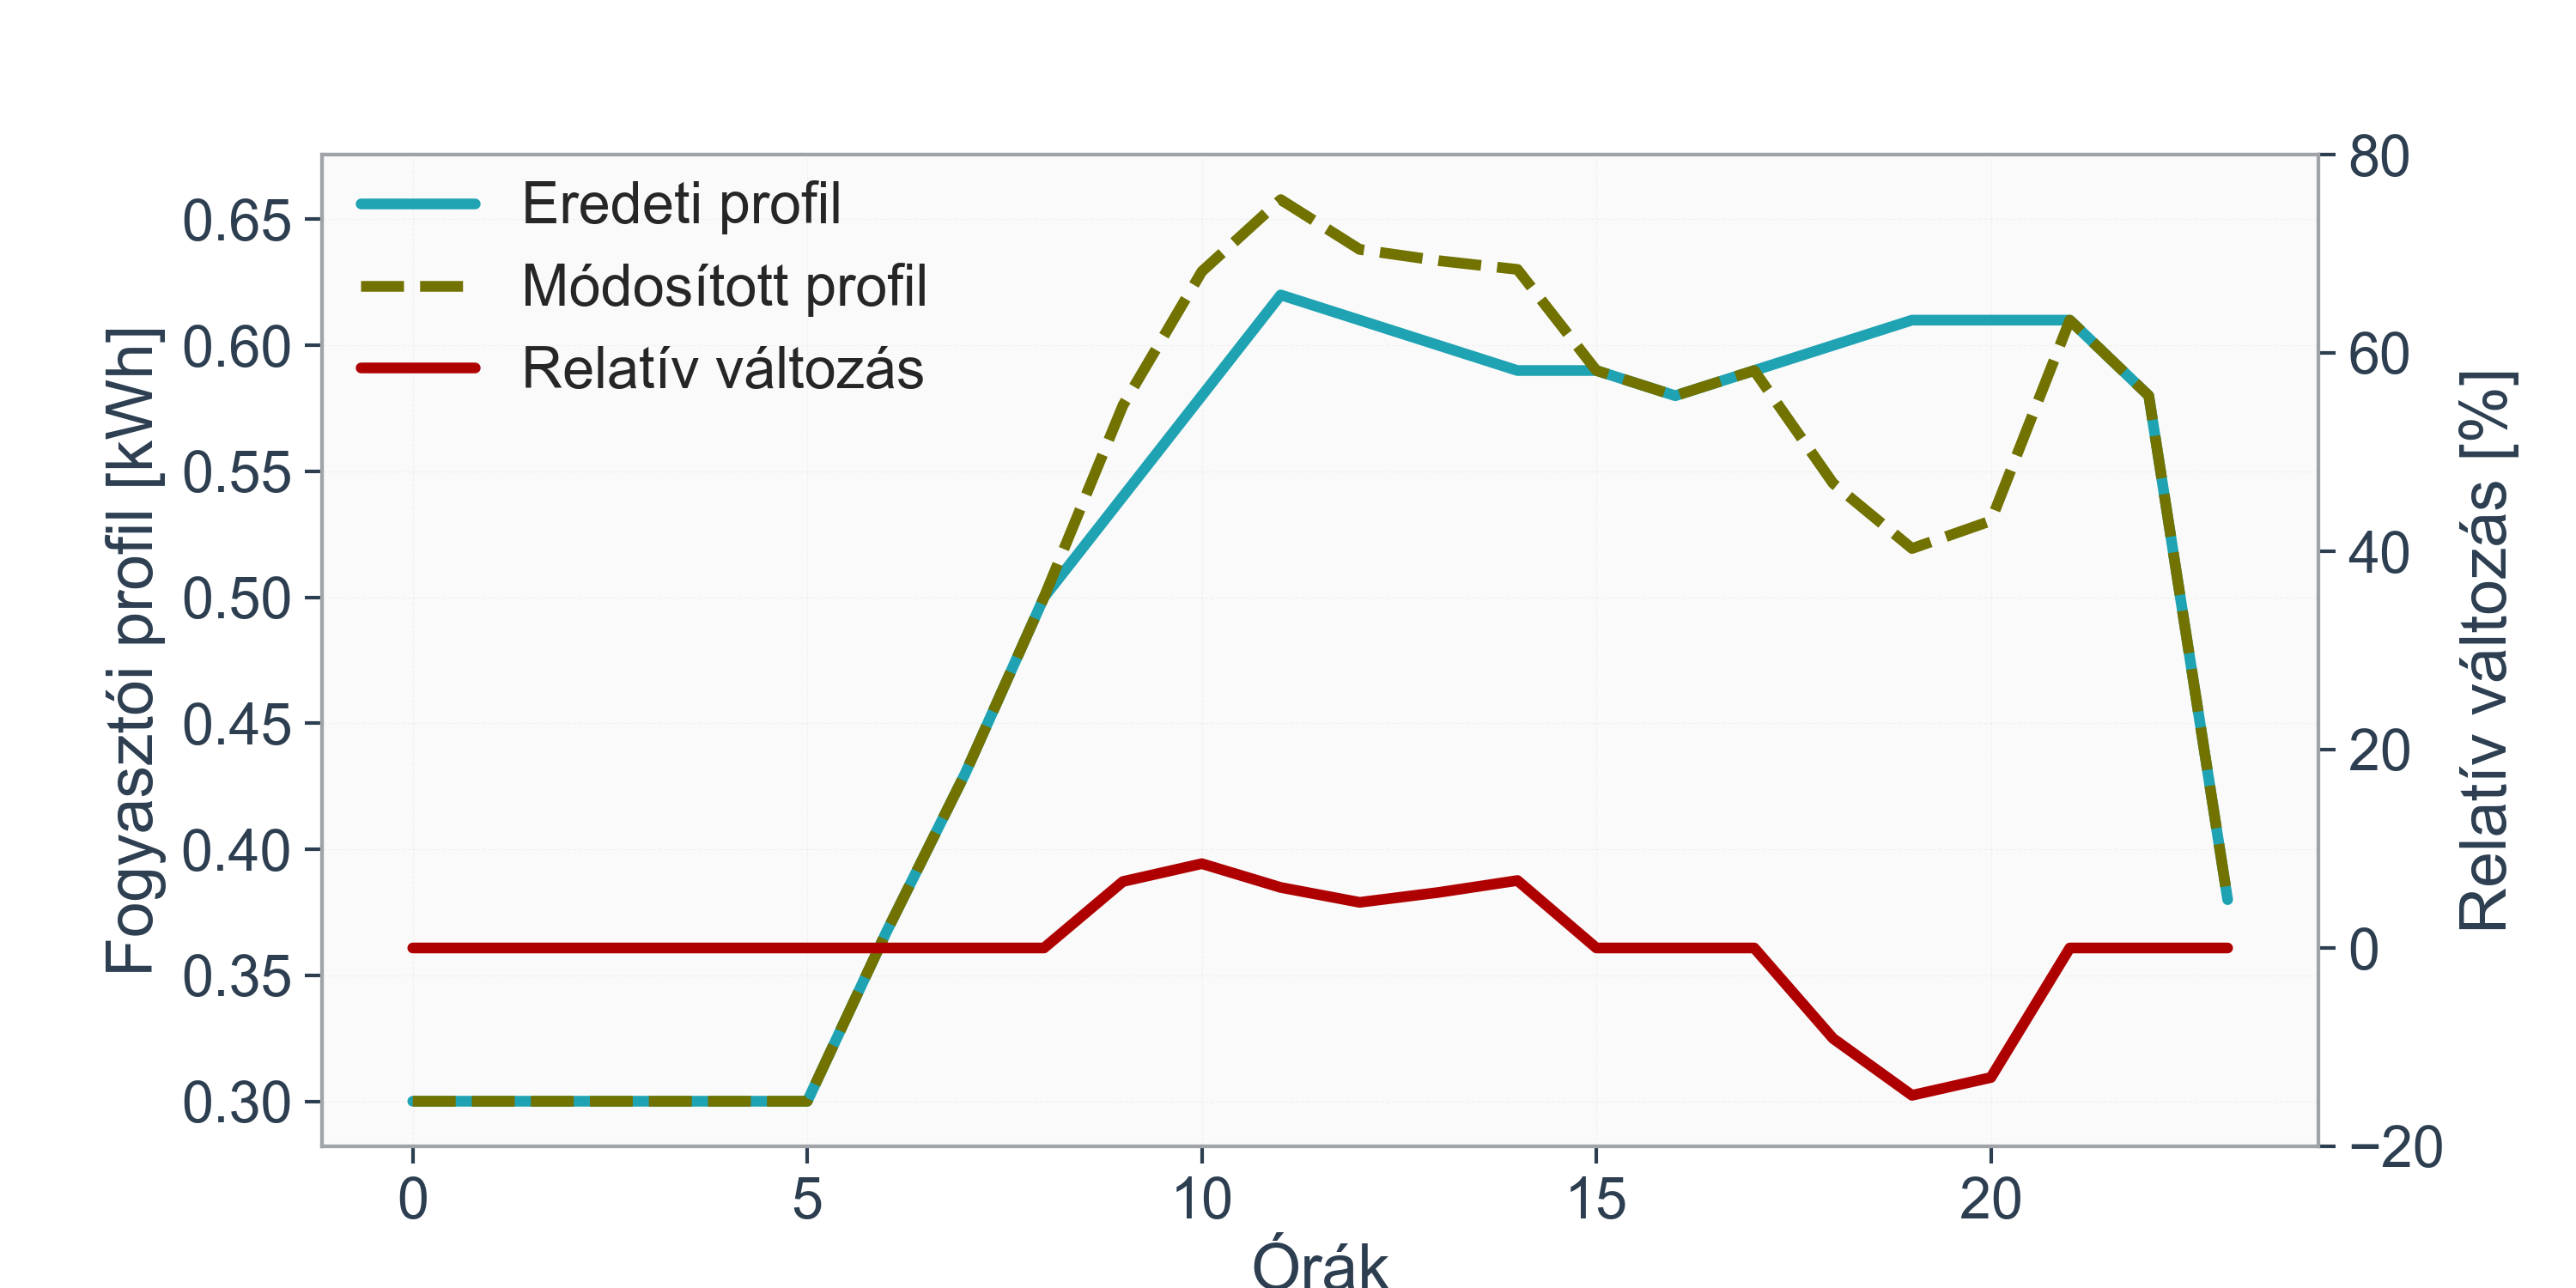
\includegraphics[width=1.2\linewidth]{figures/appliance_profile.png}
\end{minipage}

\begin{spacing}{0.7}
$^1$ \footnotesize Rollo, Antonino, et al.~"Load Shifting and Demand-Side Management in Renewable Energy Communities: Simulations of Different Technological Configurations." Energies (19961073) 18.4 (2025).
\end{spacing}
\end{frame}

\begin{frame}{Épületgépészeti rendszer modellezése}
\hspace{-1.5em}\begin{minipage}[]{0.45\columnwidth}
\small
\begin{itemize}
    \item DesignBuilder szimuláció
    \item \highlight{Air-to-water}: fűtés, hűtés és HMV, \SI{200}{l} puffertárolóval
    \item \highlight{Air-to-air}: fűtés és hűtés HP, HMV külön villanybojlerrel (\SI{120}{l}).
    \item \highlight{``SG Ready''}; setpoint módosítás napközben
    \item Egyszerű, komplex ütemezési szcenáriók
\end{itemize}
\end{minipage}
\hspace{-1em}
\begin{minipage}[]{0.5\columnwidth}
\small
\centering
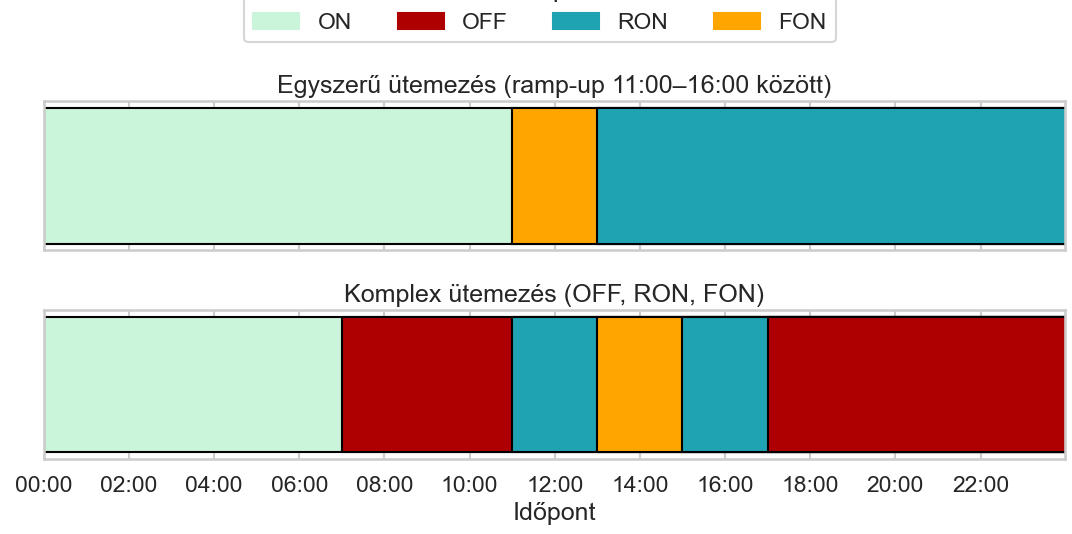
\includegraphics[width=1.2\columnwidth]{figures/scheduling.png}
\end{minipage}
\end{frame}

\begin{frame}{Használatimelegvíz-profilok}
\begin{minipage}{0.55\columnwidth}
    \begin{itemize}\setlength{\itemsep}{1.5ex}
    \item Smart mért, B-tarifás adatok alapján
    \item 59, 126, 225 l/nap/háztartás, \SI{40}{°C} csapolási hőmérséklet
    \item Szcenáriók: \highlight{reggeli} és \highlight{esti} csúcs
    \item Időbeli eloszlás: DHWcalc ajánlások szerint, napi variációval
    \item Tárolás: \SI{120}{l} HMV-tároló
\end{itemize}
\end{minipage}
\hfill
\begin{minipage}{0.35\columnwidth}
\centering
    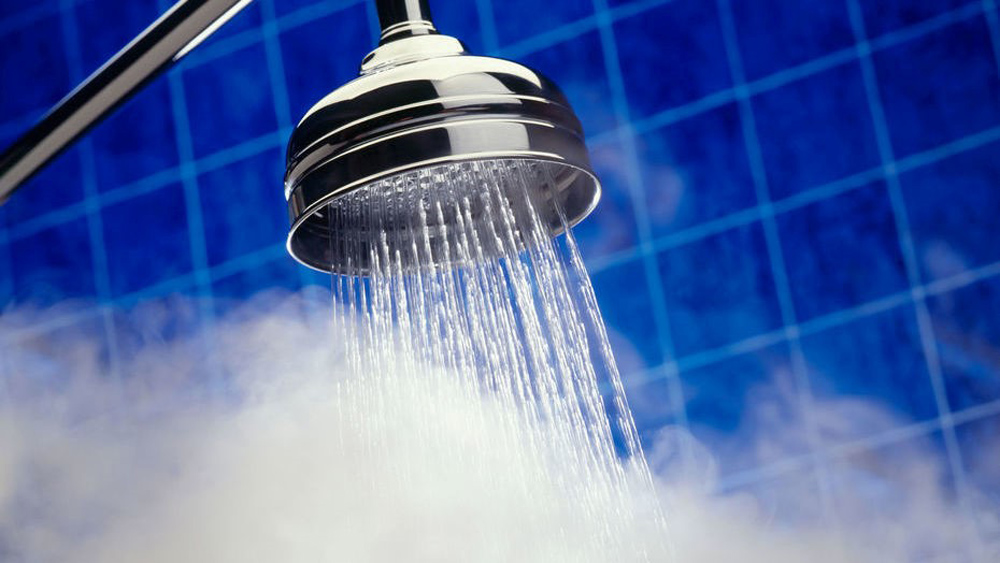
\includegraphics[width=\columnwidth]{figures/domestic_hot_water_systems.jpg}
\end{minipage}
\end{frame}

\begin{frame}{Akkumulátoros energiatároló modellje}
\hspace{-1em}\begin{minipage}[]{0.45\columnwidth}
    \centering
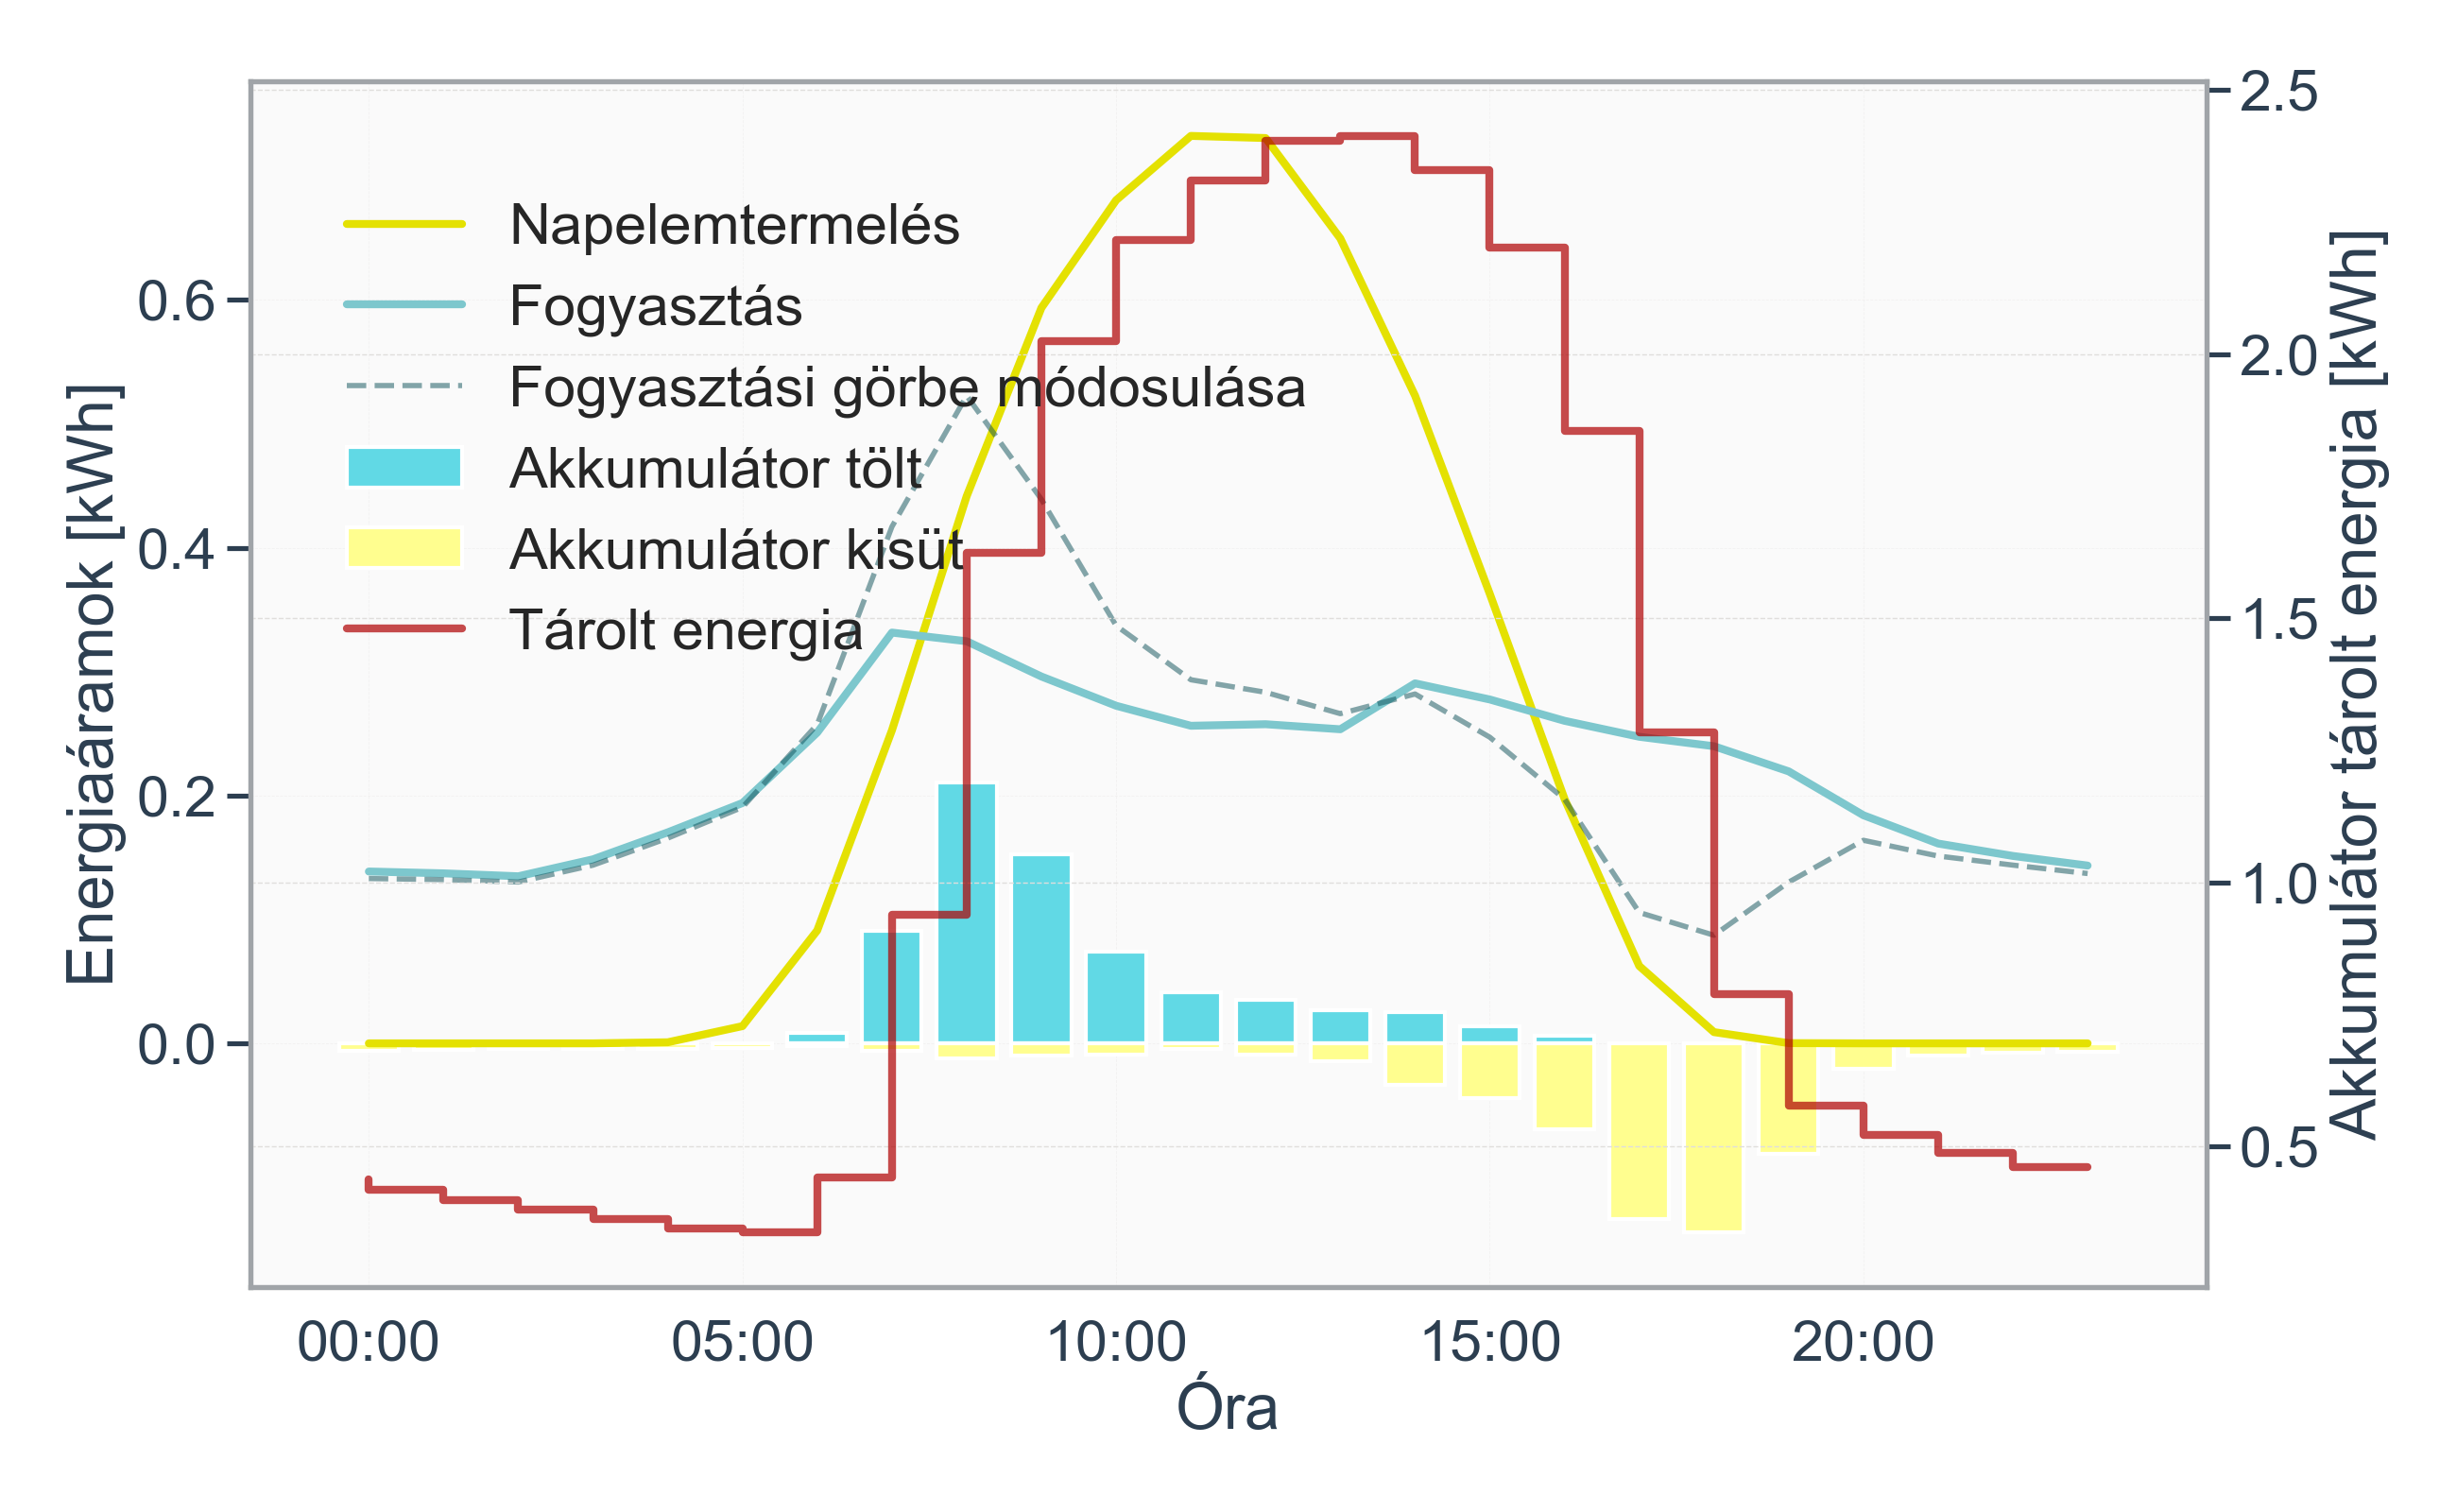
\includegraphics[width=1.2\columnwidth]{figures/battery.png}

\scriptsize
\SI{2}{kWh/kWp}, GTDR=\SI{1.5}{kWh/kWh}
\end{minipage}
\hspace{3em}
\begin{minipage}[]{0.45\columnwidth}
\begin{itemize}\setlength{\itemsep}{1.5ex}
    \item Méretezés: \{0,0.5,1,2\} kWh/kWp
    \item Hatásfok: 92\%, SOC: 10–90\%  
    \item Működés:
    \begin{itemize}
        \item PV-felesleg $\rightarrow$ betáplálás,  
        \item fogyasztás > PV $\rightarrow$ kisütés,  
        \item alacsony SOC $\rightarrow$ hálózatról tölt
    \end{itemize}
\end{itemize}
\end{minipage}
\end{frame}

\begin{frame}{Egyidejűségi metrikák}

\hspace{-1em}\begin{minipage}{0.55\columnwidth}
\begin{center}
\scriptsize
\pgfplotstableread[col sep = comma]{data/profile.csv}\datatable
\begin{tikzpicture}[remember picture]
\begin{axis}[
    width=0.95\columnwidth,
	ymin=0,
	enlarge x limits=-0.01,
	xmin=2021-07-19 01:00,
	xmax=2021-07-19 23:00,
	date coordinates in=x,
	%xlabel={2021-07-19},
	ylabel={Energia [$\si{kWh}$]},
	date ZERO=2021-07-19, 
	xticklabel=\hour:\minute,
	height=6cm,
    xtick pos=left,
	ytick pos=left,
	scaled x ticks=false,
	legend pos=outer north east,
    legend columns=2
]
	    % x-axis baseline
	\path[name path=axx] (axis cs:2021-07-19 00:00,0) -- (axis cs:2021-07-19 23:45,0);

    % Household consumption (f)
    \addplot [name path=f, thick, mediumblue2,forget plot] 
        table [x=Datetime,y=Residential, col sep=comma] {\datatable};

    % PV production (pv)
    \addplot [name path=pv, thick, yellow2,forget plot] 
        table [x=Datetime,y=PV_tmy, col sep=comma] {\datatable};

    % Consumption area (blue fill)
    \addplot[fill=lightblue, fill opacity=0.5] 
        fill between[of=f and axx];

    % PV area (yellow fill)
    \addplot[fill=yellow1, fill opacity=0.5] 
        fill between[of=pv and axx];

    % Shared energy
    \addplot[fill=lightgreen, fill opacity=0,forget plot] 
        fill between[of=pv and f];
    
    \legend{Háztartás fogyasztása, Napelemtermelés};
    % put this *before* \end{axis}
    \addlegendimage{area legend, fill=lightgreen, draw=black};
    \addlegendentry{Önfogyasztás};
\end{axis} 
\end{tikzpicture}
\end{center}
\end{minipage}
\hspace{-2.5em}
\begin{minipage}{0.5\columnwidth}
\vspace{7ex}
{
\footnotesize
\begin{itemize}
        \item Önfogyasztási index: $SCI = \frac{E_{\text{PV,used}}}{E_{\text{PV,gen}}}$
        \item Önellátási index: $SSI = \frac{E_{\text{PV,used}}}{E_{\text{load}}}$
        \item Öntermelési arány: $SP = \frac{E_{\text{PV,used}}}{E_{\text{PV,used}}+E_{\text{grid,in}}+E_{\text{grid,out}}}$
        \item Hálózathasználati tényező: $GI = \frac{E_{\text{grid,in}} + E_{\text{grid,out}}}{E_{\text{PV,used}}+E_{\text{grid,in}}+E_{\text{grid,out}}}$
    \end{itemize}
    }
\end{minipage}
\end{frame}

\section{Eredmények}
\begin{frame}{DSM hatása az önfogyasztásra}
\begin{minipage}[]{0.38\columnwidth}
\begin{itemize}\setlength{\itemsep}{2ex}
    \item Alapmodell SC $\approx 0.3$
    \item Berendezések: +2–3\%
    \item Melegvíz+épületgépészet: +5\%
    \item Akkumulátor: +40\% (mérettől függően)
\end{itemize}    
\end{minipage}
\hspace{1em}
\begin{minipage}{0.53\columnwidth}
    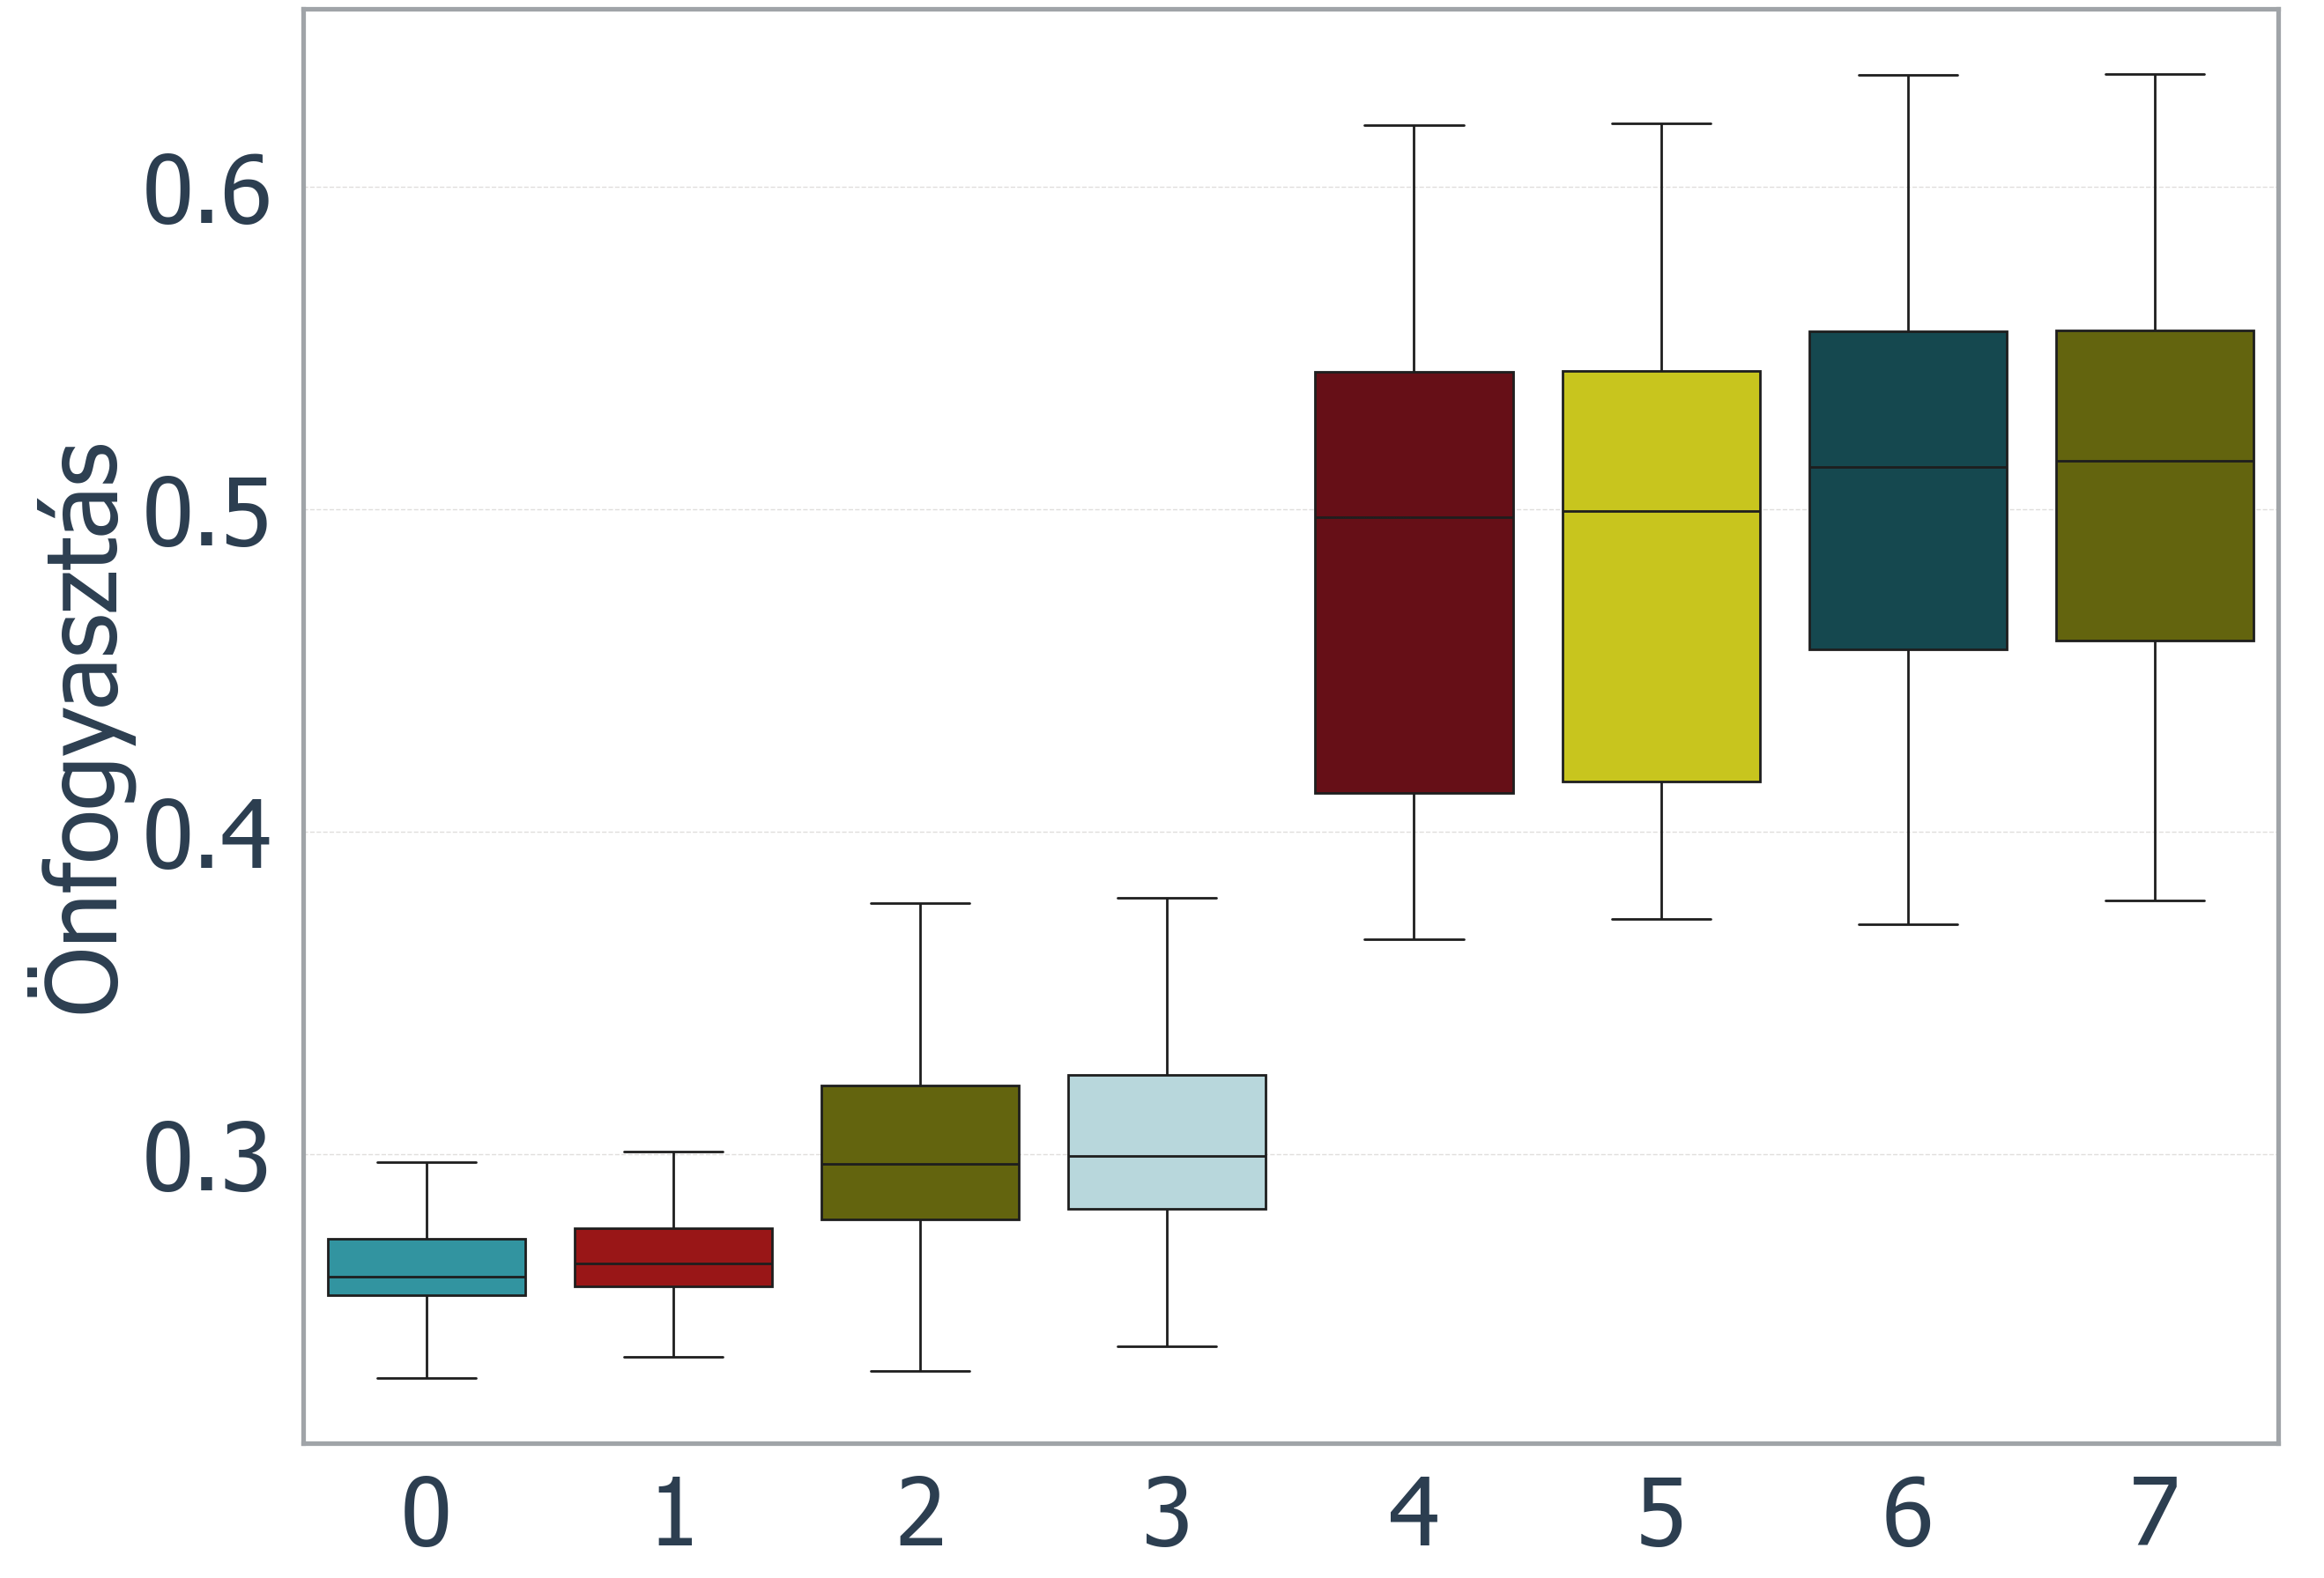
\includegraphics[width=\textwidth]{figures/dsm_id_quant.png}
\end{minipage}
\end{frame}


\begin{frame}{DSM hatása az önfogyasztásra}
\begin{center}
    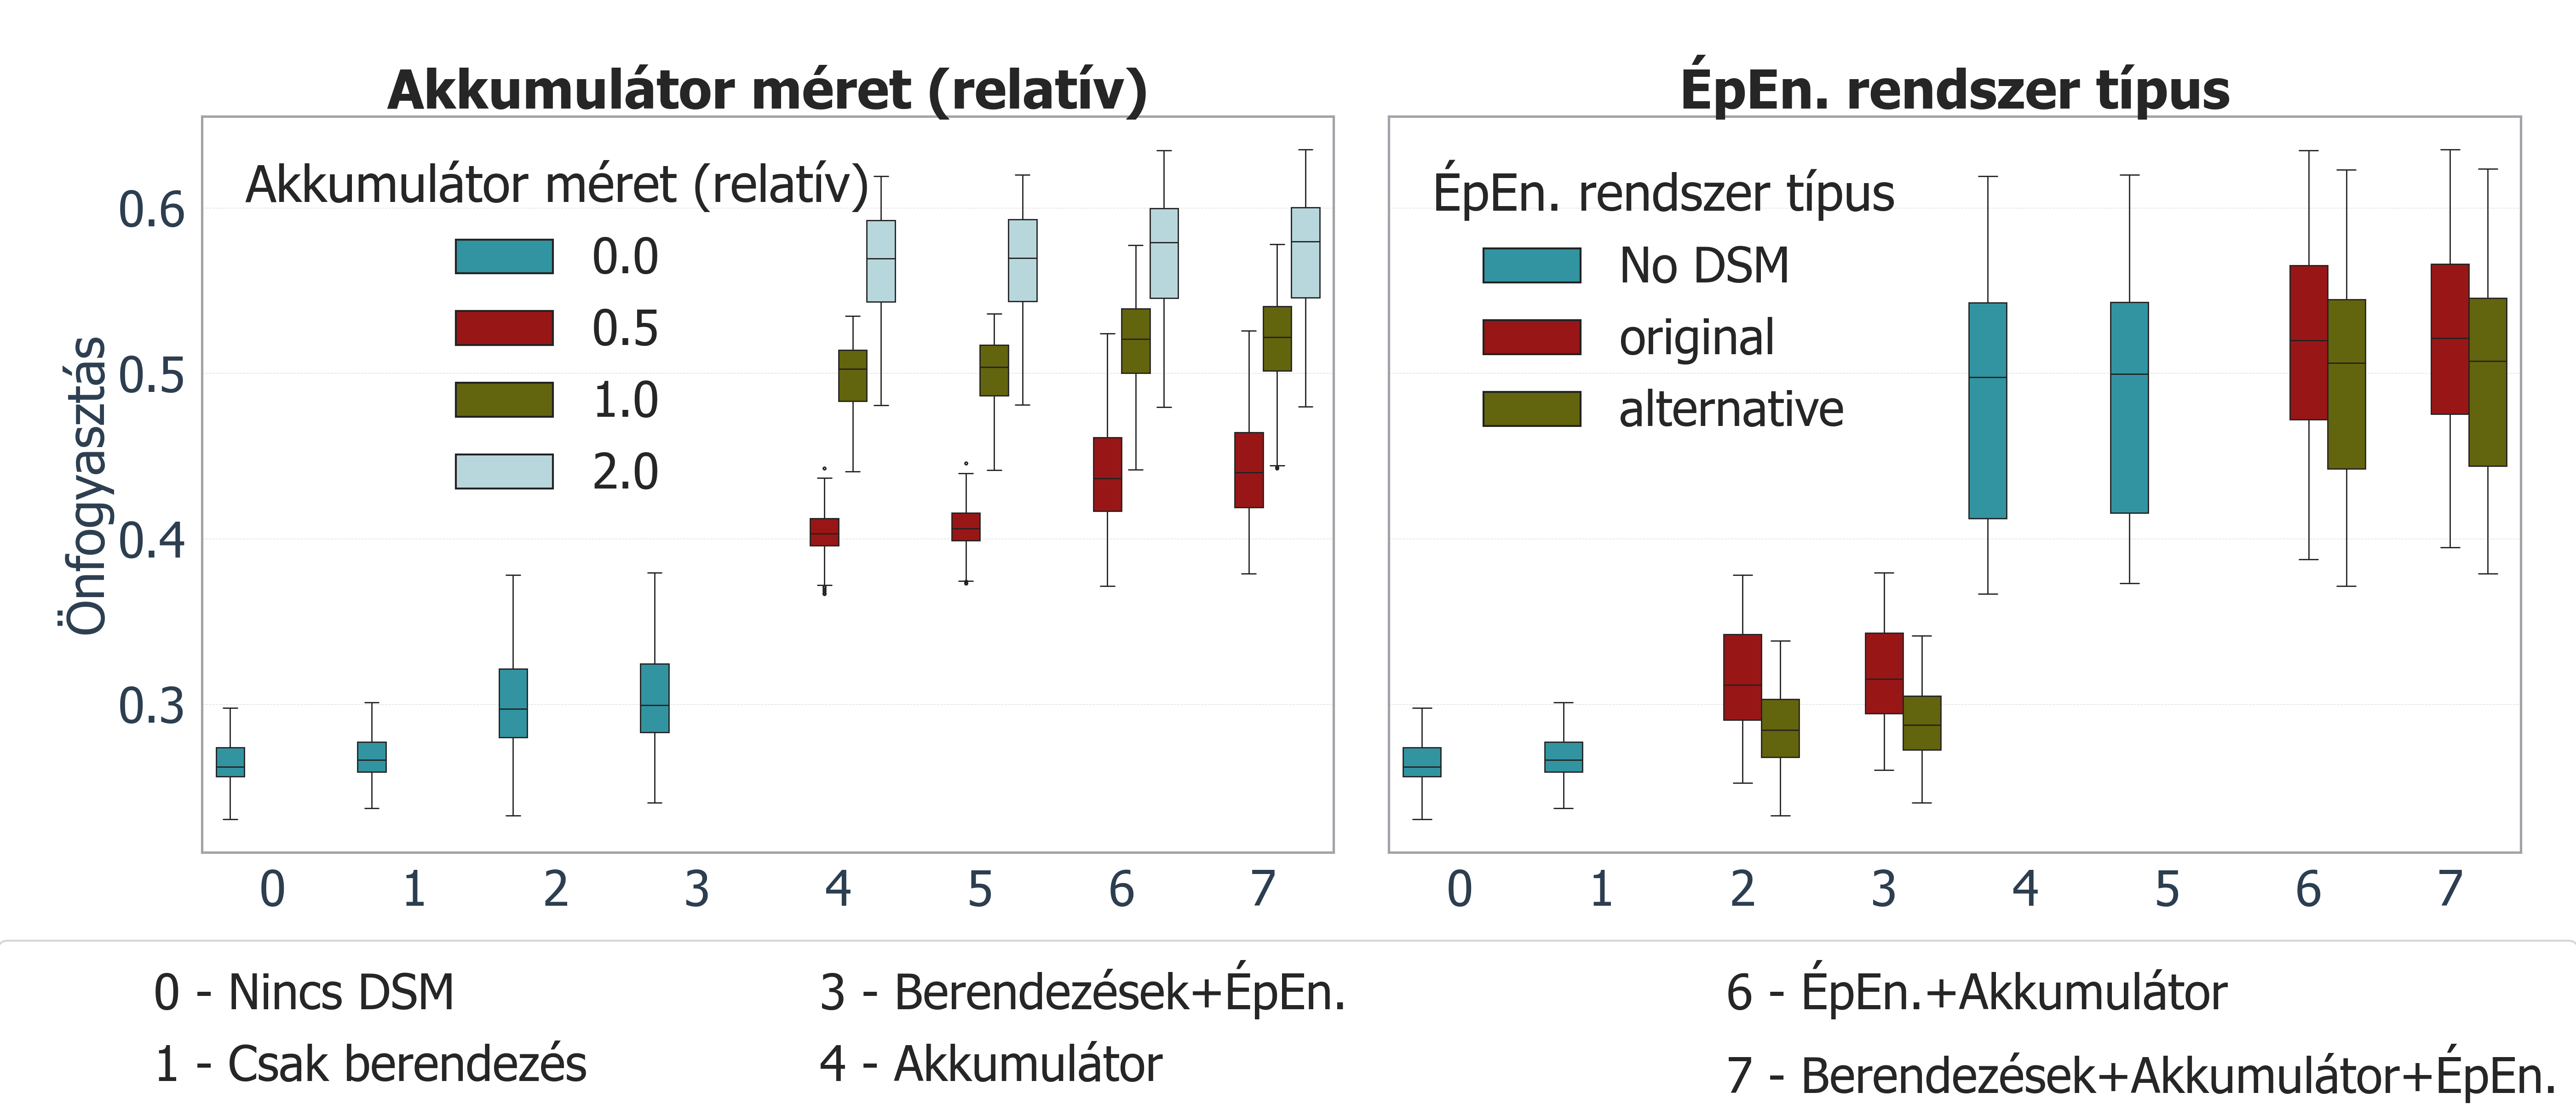
\includegraphics[width=0.85\textwidth]{figures/sc_boxplot_hu.png}
\end{center}
\end{frame}


\begin{frame}{Éves megtakarítás}
\vspace{-1ex}

\hspace{-1em}\begin{minipage}[]{0.35\textwidth}
\begin{itemize}\setlength{\itemsep}{2ex}
    \item Berendezések napközbeni használata: kb.~10,000 Ft
    \item Épületgépészeti rendszer időzítése: kb.~25,000 Ft
    \item Akkumulátoros tárolás: 170,000 Ft
\end{itemize}    
\end{minipage}
\hspace{2em}
\begin{minipage}[]{0.55\textwidth}
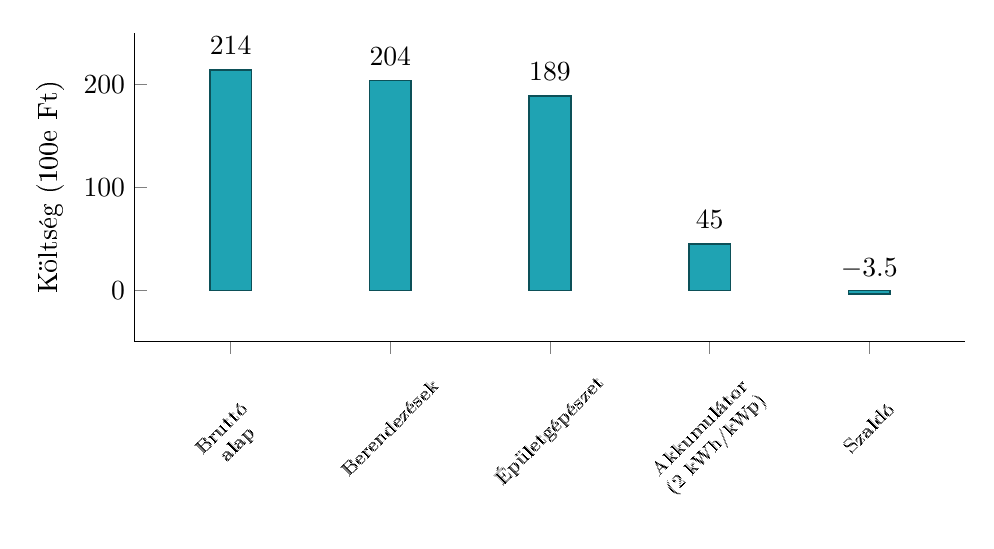
\begin{tikzpicture}[remember picture]
\begin{axis}[
    ybar,
    bar width=15pt,
    ymin=-50, ymax=250,
    ylabel={Költség (100e Ft)},
    symbolic x coords={Bruttó\\alap,Berendezések,Épületgépészet,Akkumulátor\\(2 kWh/kWp),Szaldó},
    xtick=data,
    x tick label style={font=\scriptsize,text width=2cm,align=center,rotate=45},
    nodes near coords,
    every node near coord/.append style={
        font=\bfseries,
        anchor=south,
        yshift=2pt
    },
    axis x line*=bottom,
    axis y line*=left,
    width=\textwidth,
    height=5.5cm,
    enlarge x limits=0.15
]

\addplot[fill=mediumblue,draw=mediumblue2,line width=0.6pt] coordinates {
    (Bruttó\\alap,214)
    (Berendezések,204)
    (Épületgépészet,189)
    (Akkumulátor\\(2 kWh/kWp),45)
    (Szaldó,-3.5)
};

\end{axis}
\end{tikzpicture}
\end{minipage}
\end{frame}

\section{}
\begin{frame}[endframe,noframenumbering]{}

\hspace{-1.5em}{\Large \color{mediumblue2} Összegzés}
\vspace{1.5ex}

\hspace{-1.5em}\begin{minipage}[b]{0.5\textwidth}
\begin{itemize}
    \item DSM több tízezer Ft megtakarítást eredményezhet
    \item Akkumulátor drága, de kiemelkedő hatású
    \item DSM + Akkumulátor kombináció: optimális megoldás
    \item A DSM hálózati szempontból is kedvezőbb
\end{itemize}
\end{minipage}
\hspace{5em}
\begin{minipage}[b]{0.32\textwidth}
\centering


\includegraphics[width=0.7\columnwidth]{figures/qr.png}

\url{https://www.hmke.info/kalkulatorok}
\end{minipage}

\vspace{2.5ex}
{\Large \color{lightblue2} Köszönjük a figyelmet!}

\vspace{1ex}
{\scriptsize barancsuk.lilla$@$ek.hun-ren.hu}
\end{frame}

\end{document}